The main idea of the inception network is to approximate an optimal local sparse network by dense components. An optimal local sparse network can be constructed layer by layer. 
For each layer, the correlation statistics of the last layer are clustered into groups of high correlation. These clusters form the units of the layer and are connected to the units of the previous layer. 
This can be imagined in terms of the Hebbian principle (\enquote{what fires together, wires together}). Neurons in a correlation cluster (\enquote{what fires together}) are connected to neurons in another correlation cluster (\enquote{wires together}).
Clusters concentrated in a narrow region can be covered by a convolution of small size. Clusters concentrated in a wider region can be covered by a convolution of a bigger size. \autocite{Szegedy.2015}
\par
Inception networks approximate the optimal local sparse network by combining those convolutions. The convolutions are combined in inception modules. The naive version of an inception module combines max pooling and three convolutional layers with kernel size $1$, $3$, and $5$. These are applied in parallel to the input of the inception module. This way, the inception module is branched into four distinct paths. The resulting activation maps are concatenated to one output. That way, the four paths are merged into one output. This output is the output of the inception module. The input of the inception module is an array of channels. This naive version of the inception module is illustrated in Figure \ref{fig:naiveinceptionmodule}. \autocite{Szegedy.2015}
\begin{figure}[H]
	\centering
	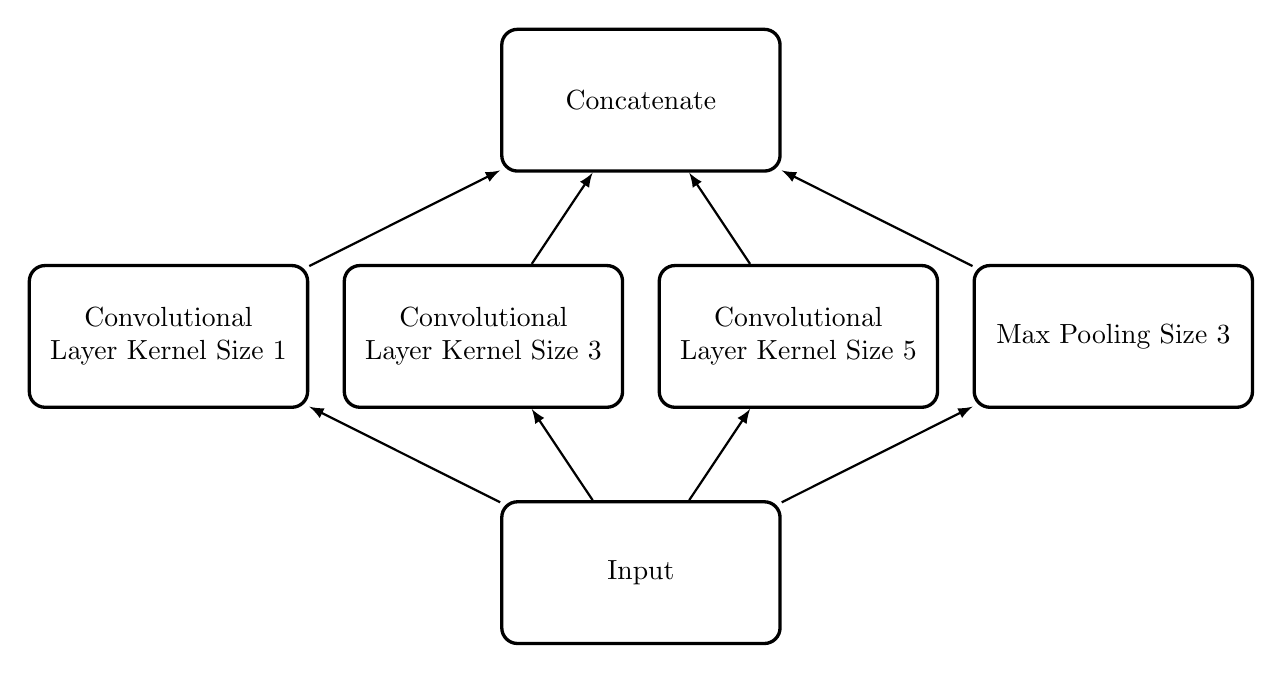
\begin{tikzpicture}[
	cell/.style={
		rectangle, 
		rounded corners=2mm, 
		draw,
		very thick,
		align=center,
		text width=3.3cm,
		minimum height=1.8cm
	},
	ArrowC1/.style={% Arrows with rounded corners
		rounded corners=.25cm,
		thick,
	},
]
	\node [cell] (out) at (0,6) {Concatenate};

	\node [cell] (c1) at (-6,3) {Convolutional Layer Kernel Size $1$};
	\node [cell] (c3) at (-2,3) {Convolutional Layer Kernel Size $3$};
	\node [cell] (c5) at (2,3) {Convolutional Layer Kernel Size $5$};
	\node [cell] (p) at (6,3) {Max Pooling Size $3$};
	
	\node [cell] (in) at (0,0) {Input};
	
	\draw [-latex,ArrowC1] (in) -- (c1);
	\draw [-latex,ArrowC1] (in) -- (c3);
	\draw [-latex,ArrowC1] (in) -- (c5);
	\draw [-latex,ArrowC1] (in) -- (p);
	\draw [-latex,ArrowC1] (c1) -- (out);
	\draw [-latex,ArrowC1] (c3) -- (out);
	\draw [-latex,ArrowC1] (c5) -- (out);
	\draw [-latex,ArrowC1] (p) -- (out);
\end{tikzpicture}
	\caption{Naive Inception Module (own figure)} \label{fig:naiveinceptionmodule}
\end{figure}
Inception networks are neural networks containing inception modules. The naive version of inception modules increases the number of outputs. Accordingly, stacking inception modules leads to a rapid increase of computational complexity. Thus, the number of outputs is reduced by dimension reduction. Dimension reduction is computed by convolutions of kernel size $1$. This convolution is applied before the computationally expensive convolutions of kernel size $3$ and $5$ as well as after max pooling. The resulting inception module is illustrated in Figure \ref{fig:inceptionmodule}. \autocite{Szegedy.2015}
\begin{figure}[H]
	\centering
	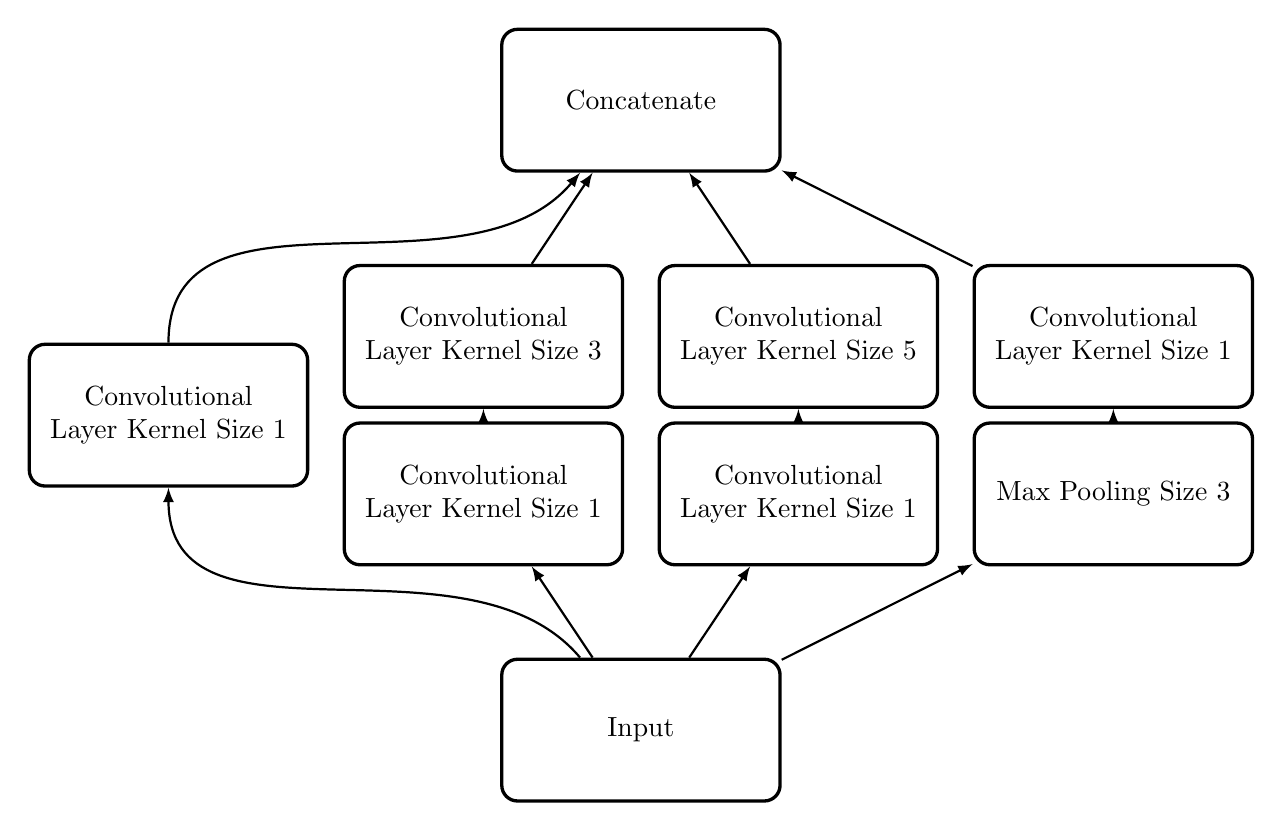
\begin{tikzpicture}[
	cell/.style={
		rectangle, 
		rounded corners=2mm, 
		draw,
		very thick,
		align=center,
		text width=3.3cm,
		minimum height=1.8cm
	},
	ArrowC1/.style={% Arrows with rounded corners
		rounded corners=.25cm,
		thick,
	},
]
	\node [cell] (out) at (0,8) {Concatenate};

	\node [cell] (c1) at (-6,4) {Convolutional Layer Kernel Size $1$};
	
	\node [cell] (c3) at (-2,5) {Convolutional Layer Kernel Size $3$};
	\node [cell] (c5) at (2,5) {Convolutional Layer Kernel Size $5$};
	\node [cell] (cp) at (6,5) {Convolutional Layer Kernel Size $1$};
	
	\node [cell] (c13) at (-2,3) {Convolutional Layer Kernel Size $1$};
	\node [cell] (c15) at (2,3) {Convolutional Layer Kernel Size $1$};
	\node [cell] (p) at (6,3) {Max Pooling Size $3$};
	
	
	\node [cell] (in) at (0,0) {Input};
	
	\draw [-latex,ArrowC1] (in) to[out=130,in=-90] (c1);
	\draw [-latex,ArrowC1] (in) -- (c13);
	\draw [-latex,ArrowC1] (in) -- (c15);
	\draw [-latex,ArrowC1] (in) -- (p);
	
	\draw [-latex,ArrowC1] (c13) -- (c3);
	\draw [-latex,ArrowC1] (c15) -- (c5);
	\draw [-latex,ArrowC1] (p) -- (cp);
	
	\draw [-latex,ArrowC1] (c1) to[out=90,in=-130] (out);
	\draw [-latex,ArrowC1] (c3) -- (out);
	\draw [-latex,ArrowC1] (c5) -- (out);
	\draw [-latex,ArrowC1] (cp) -- (out);
\end{tikzpicture}
	\caption{Inception Module (own figure)} \label{fig:inceptionmodule}
\end{figure}
Based on this, inception modules can be generalized. A generalized inception module is comprised of several paths. The paths branch from the input of the inception module and merge to the output of the inception module. \autocites{Szegedy.2016}{Szegedy.2017}{Xie.2017}
\par
The best-performing inception network found in the course of the literature review is the $101$ version of \cite{Xie.2017}'s ResNeXt, called ResNeXt-101. This version is based on the $101$-layer version of ResNet.
The input of ResNeXt-101 is a $224$-by-$224$-pixel, \ac{RGB} image. The output of ResNeXt-101 comprises the probabilities of the $c$~target classes. \autocite{Xie.2017}
\par
ResNeXt-101 is comprised of convolutional layers followed by $1$ dense layer.
The convolutional layers have a stride of $1$, unless specified otherwise.
The convolutional layers use batch normalization and the \ac{ReLU} activation function.
Batch normalization is applied after every convolution before the activation function.
The dense layer has $c$ neurons and uses the softmax activation function.
The first convolutional layer is followed by max pooling, has a kernel size of $7$, and a stride of $2$.
Max pooling is applied with a pooling size of $3$ and a pooling stride of $2$. \autocite{Xie.2017}
\par
The remaining covolutional layers are arranged in inception modules with shortcut connections. An inception module consists of $32$ paths. A path consists of three convolutional layers. The first and third layer have a kernel size of $1$. The second layer has a kernel size of $3$. The first and third layer are used to reduce, then increase (restore) dimensions. This way, the second layer becomes a bottleneck with smaller input/output dimensions. On that account, computation costs are reduced.
The shortcut connection skips the inception module. The shortcut connection uses identity mapping. The output of the identity mapping is added element-wise to the output of the skipped inception module. The result is transformed by the \ac{ReLU} activation function. \autocite{Xie.2017}
ResNeXt-101 consists of 4 types of stacked inception modules . The types differ only in the number of kernels of their layers. The configurations of each inception module are outlined in Table \ref{tab:resnext}. \autocite{Xie.2017} 
\par
The first layer of the first block of a type has a stride of $2$ for all paths. This way, the feature map size is halved while the number of filters is doubled. Hence, the time complexity per inception module is preserved.
The last layer of the last block is followed by global average pooling. \autocite{Xie.2017}
\par
The whole configuration of ResNeXt-101 is outlined in Table \ref{tab:resnext}. \autocite{Xie.2017}
\begin{xltabular}{\textwidth}{lX}\toprule
	\caption[ResNeXt-101 Configuration]{ResNeXt-101 Configuration. Note that each $k \times k \text{ conv } K$ denotes a convolutional layer with $K$ kernels of size  $k$. An inception module is denoted as an array of layers and $P=p$ with $p$ being the number of paths.
	} \label{tab:resnext}\\
	\textbf{Layer/Module} & \textbf{Configuration}\\\midrule \endhead
	Input Layer & $7 \times 7, 64$ with stride of $2$, and $3 \times 3$ max pooling with stride of $2$\\\midrule
	Inception Modul $1-3$ & $\begin{bmatrix}
	1 \times 1 \text{ conv } 4 & \\
	3 \times 3 \text{ conv } 4 & P=32\\
	1 \times 1  \text{ conv } 256 &
	\end{bmatrix} \times 3$\\\midrule
	Inception Modul $4-7$ & $\begin{bmatrix}
	1 \times 1 \text{ conv } 4 &\\
	3 \times 3 \text{ conv } 4 & P=32\\
	1 \times 1 \text{ conv } 512 &
	\end{bmatrix} \times 4$\\\midrule
	Inception Modul $8-30$ & $\begin{bmatrix}
	1 \times 1 \text{ conv } 4 &\\
	3 \times 3 \text{ conv } 4 & P=32\\
	1 \times 1 \text{ conv } 1024 &
	\end{bmatrix} \times 23$\\\midrule
	Inception Modul $31-33$ & $\begin{bmatrix}
	1 \times 1 \text{ conv } 4 &\\
	3 \times 3 \text{ conv } 4 & P=32\\
	1 \times 1 \text{ conv } 2048 &
	\end{bmatrix} \times 3$\\\midrule
	Output Layer & global average pooling, dense with $c$ neurons
	\\\bottomrule
\end{xltabular}
